\subsection{Backend Arkitektur}
\label{ssec: BackendArkitektur}
I dette afsnit gives en redegørelse for backendens arkitektur samt formål.\\ 
 
\noindent Backend containeren består overordnet set af to dele et Web Api og en database, i dette afsnit vil fokusset ligge på Web Api'et for flere detaljer omkring databasens arkitektur henvises til afsnit \textbf{Mangler ref til db ark}. Web Api'et vil blive udviklet i frameworket ASP.NET Core. Web api'et skal kunne tilgåes af clienter igennem HTTP request/responses, for at hente/sende gemte spil. Web api'et kontakter efterfølgende databasen igennem et DAL, som udfører de nødvendige queries. Hertil skal Web api'et sørge for Authentication og Authorization den bruger som er logget ind på clienten hvorfra der kaldes. \\

\noindent Til at beskrive backendens arkitektur udarbejdes et C4 level 3 diagram. Diagrammet som kan ses på \autoref{fig:Arkitektur-Backend-C3} giver et overblik over hvilke componenter backenden består af, hvilke teknologier det forventes at anvende, samt hvordan de kommunikerer indbyrdes og med resten af systemet.\\

 
\begin{figure}[H]
\centering
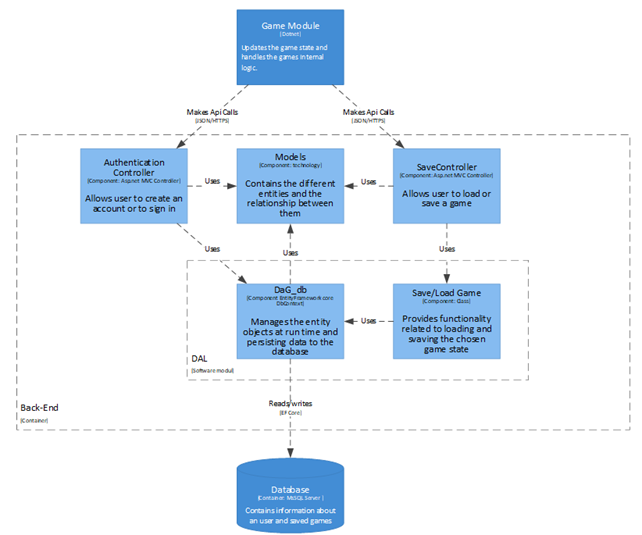
\includegraphics[width = \textwidth]{02-Body/Images/Backend_C3.PNG}
\caption{C3-Model over Backend container,figuren giver et overblik over de componenter backenden består, samt hvordan disse kommunikere indbyrdes og med omkring liggende containere.}
\label{fig:Arkitektur-Backend-C3}
\end{figure}

\noindent Figuren illustrerer en lagdelt struktur, som gør brug af MVC mønstret. Der ses en client (Game Module) som kalder ned i to controllere Authentication og Save Controller. Kommunikationen her i mellem foregår med HTTPS req/resp, med dataen på JSON format.\\

\noindent \textbf{Controller:}\\
Controllerne opdeles efter ansvar såldes der er en som står for bruger håndtering og en som står for at gemme/hente spil. Disse vil bestå af ASP.Net MVC Controllere \cite{MVC controller}.

\noindent \textbf{DAL:}\\
De to controllere kalder videre ned i DAL laget, som består af en database kontekst og en klasse til at håndtere queries for SaveControlleren. Til at skabe denne database kontekst anvendes EF Core \cite{EF Core}.

\noindent \textbf{Model:}\\
Modellerne fungerer som bindeledet mellem alle komponenterne, de definerer den data som der arbejdes på, og vil bestå af en række C\# klasser.\\

\noindent MVC mønstret bidrager med at skabe højere samhørighed i applikationen ved at muliggøre en logisk opdelling af funktionalitet i controllerne, ved at de tager ansvar for hver deres områder af kommunikationen (Bruger og spil). Dets ses også at koblingen mellem modulerne er forholdsvis lav såldes, således det er let at bygge videre på og tilføje ny funktionalitet uden at ødelægge noget.\\

\subsubsection{REST}
I designet af Web Api'et søges det at opnå følgende 5 REST principper \cite{REST}.

\begin{enumerate}
 \item Alle de data objekter der arbejdes med tilhører en bestemt unique URI. Dataen hentes, sendes og manipuleres igennem standard HTTP metoder som (GET, POST, PUT, DELETE).
 \item Der arbejdes ud fra en client/server arkitektur med data som resource. 
 \item Web Api’et er stateless, hvilket vil sige der gemmes ikke nogen tilstand omkring clienten på server siden.
 \item Der arbejdes ud fra en lagdelt struktur, som betyder at hver component kun kan se de componenter som grænser op til den selv.
 \item Der anvendes Cashing på server siden (Dette vil ikke blive implementeret).
\end{enumerate}

\noindent Dette bidrager til at data overførelserne ikke bliver for komplekse og for at overholde SoC, ved at adskille repræsentationen og dataen fra hinanden.

\subsubsection{Konlusion}

Systemets backend består at Web Api, som bygges op omkring MVC mønstret, Web Api’et vil gøre brug af REST principper for at adskille data resourcerne fra deres repræsentation på clientens side.

\newpage
